\documentclass[12pt,a4paper]{article}
\usepackage[margin=1in]{geometry}
\usepackage{graphicx}
\usepackage{hyperref}
\usepackage{enumitem}
\usepackage{booktabs}
\usepackage{xcolor}
\usepackage{amssymb}
\usepackage{fancyhdr}
\usepackage{titlesec}
\usepackage{listings}
\usepackage{caption}
\usepackage{float}

\definecolor{primary}{RGB}{30,64,175}
\definecolor{codebg}{RGB}{245,245,250}
\definecolor{codetext}{RGB}{40,40,40}

\lstset{
  backgroundcolor=\color{codebg},
  basicstyle=\ttfamily\small\color{codetext},
  breaklines=true,
  frame=single,
  rulecolor=\color{gray!30},
  xleftmargin=0.5cm,
  framexleftmargin=0.5cm,
  numbers=none,
  showstringspaces=false,
}

\hypersetup{
  colorlinks=true,
  linkcolor=primary,
  urlcolor=primary,
  citecolor=primary,
}

\pagestyle{fancy}
\fancyhf{}
\fancyhead[L]{\small CSE 345/545 --- Foundations to Computer Security}
\fancyhead[R]{\small Milestone 3 Report}
\fancyfoot[C]{\thepage}
\renewcommand{\headrulewidth}{0.4pt}

\titleformat{\section}{\large\bfseries\color{primary}}{}{0em}{}
\titleformat{\subsection}{\normalsize\bfseries\color{primary!80!black}}{}{0em}{}

\begin{document}

% ============= TITLE PAGE =============
\begin{titlepage}
\centering
\vspace*{2cm}
{\Huge\bfseries\color{primary} VajraKavach\par}
\vspace{0.5cm}
{\Large Secure Job Search \& Professional Networking Platform\par}
\vspace{2cm}
{\LARGE\bfseries Project Milestone 3 Report\par}
\vspace{0.3cm}
{\large CSE 345/545: Foundations to Computer Security\par}
\vspace{2cm}

\begin{tabular}{ll}
\toprule
\textbf{Team Members} & \textbf{Roll Number} \\
\midrule
Yash Kumar Vaibhav & MT25091 \\
Aayush Gupta & MT25008 \\
Ayush Jain & MT25066 \\
Ayush Kumar & 2020290 \\
\bottomrule
\end{tabular}

\vspace{2cm}
{\large Indraprastha Institute of Information Technology, Delhi\par}
\vspace{0.3cm}
{\large March 31, 2026\par}
\vfill
\end{titlepage}

% ============= CONTENT =============
\tableofcontents
\newpage

% ============================================================
\section{Company Pages and Job Postings}
% ============================================================

\subsection{Overview}
VajraKavach allows recruiters and platform admins to create and manage company pages, and post job listings linked to those companies. All users can browse and search companies and jobs.

\subsection{Company Page Management}
\begin{enumerate}
  \item Recruiters create a company page with name, description, location, and website URL.
  \item Each company is linked to an \texttt{admin\_id} (the recruiter who created it).
  \item Companies can be searched by name and location (case-insensitive).
  \item Only the company owner or a platform admin can update or delete a company.
  \item Companies support a \texttt{is\_verified} flag for admin-verified organizations.
\end{enumerate}

\subsection{Job Posting System}
\begin{enumerate}
  \item Recruiters create job postings linked to one of their companies.
  \item Job fields include: title, description, required skills, location, salary range (optional), and application deadline.
  \item Jobs support enums for consistency:
    \begin{itemize}
      \item \textbf{Location Type:} Remote, On-site, Hybrid.
      \item \textbf{Job Type:} Full-time, Part-time, Internship, Contract.
    \end{itemize}
  \item Jobs have an \texttt{is\_active} flag allowing recruiters or admins to delist postings.
  \item Applicant count is tracked and displayed per job listing.
\end{enumerate}

\subsection{API Endpoints}
\begin{table}[H]
\centering
\begin{tabular}{lll}
\toprule
\textbf{Method} & \textbf{Endpoint} & \textbf{Access} \\
\midrule
POST & \texttt{/api/companies/} & Recruiter, Admin \\
GET & \texttt{/api/companies/search} & Authenticated \\
GET & \texttt{/api/companies/my} & Recruiter \\
PUT & \texttt{/api/companies/\{id\}} & Owner, Admin \\
DELETE & \texttt{/api/companies/\{id\}} & Owner, Admin \\
\midrule
POST & \texttt{/api/jobs/} & Recruiter, Admin \\
GET & \texttt{/api/jobs/search} & Authenticated \\
GET & \texttt{/api/jobs/my} & Recruiter \\
PUT & \texttt{/api/jobs/\{id\}} & Owner, Admin \\
DELETE & \texttt{/api/jobs/\{id\}} & Owner, Admin \\
\bottomrule
\end{tabular}
\caption{Company and Job API Endpoints}
\end{table}

\subsection{Security Measures}
\begin{itemize}
  \item \textbf{Role-Based Access Control:} Only recruiters and platform admins can create companies and post jobs.
  \item \textbf{Ownership Verification:} Modifications require company ownership or admin privileges.
  \item \textbf{Input Validation:} Pydantic schemas enforce valid data types, URL formats, and salary ranges.
  \item \textbf{Audit Logging:} All company and job CRUD operations are logged in the tamper-evident audit trail.
\end{itemize}

\subsection{Screenshots}

\begin{figure}[H]
\centering
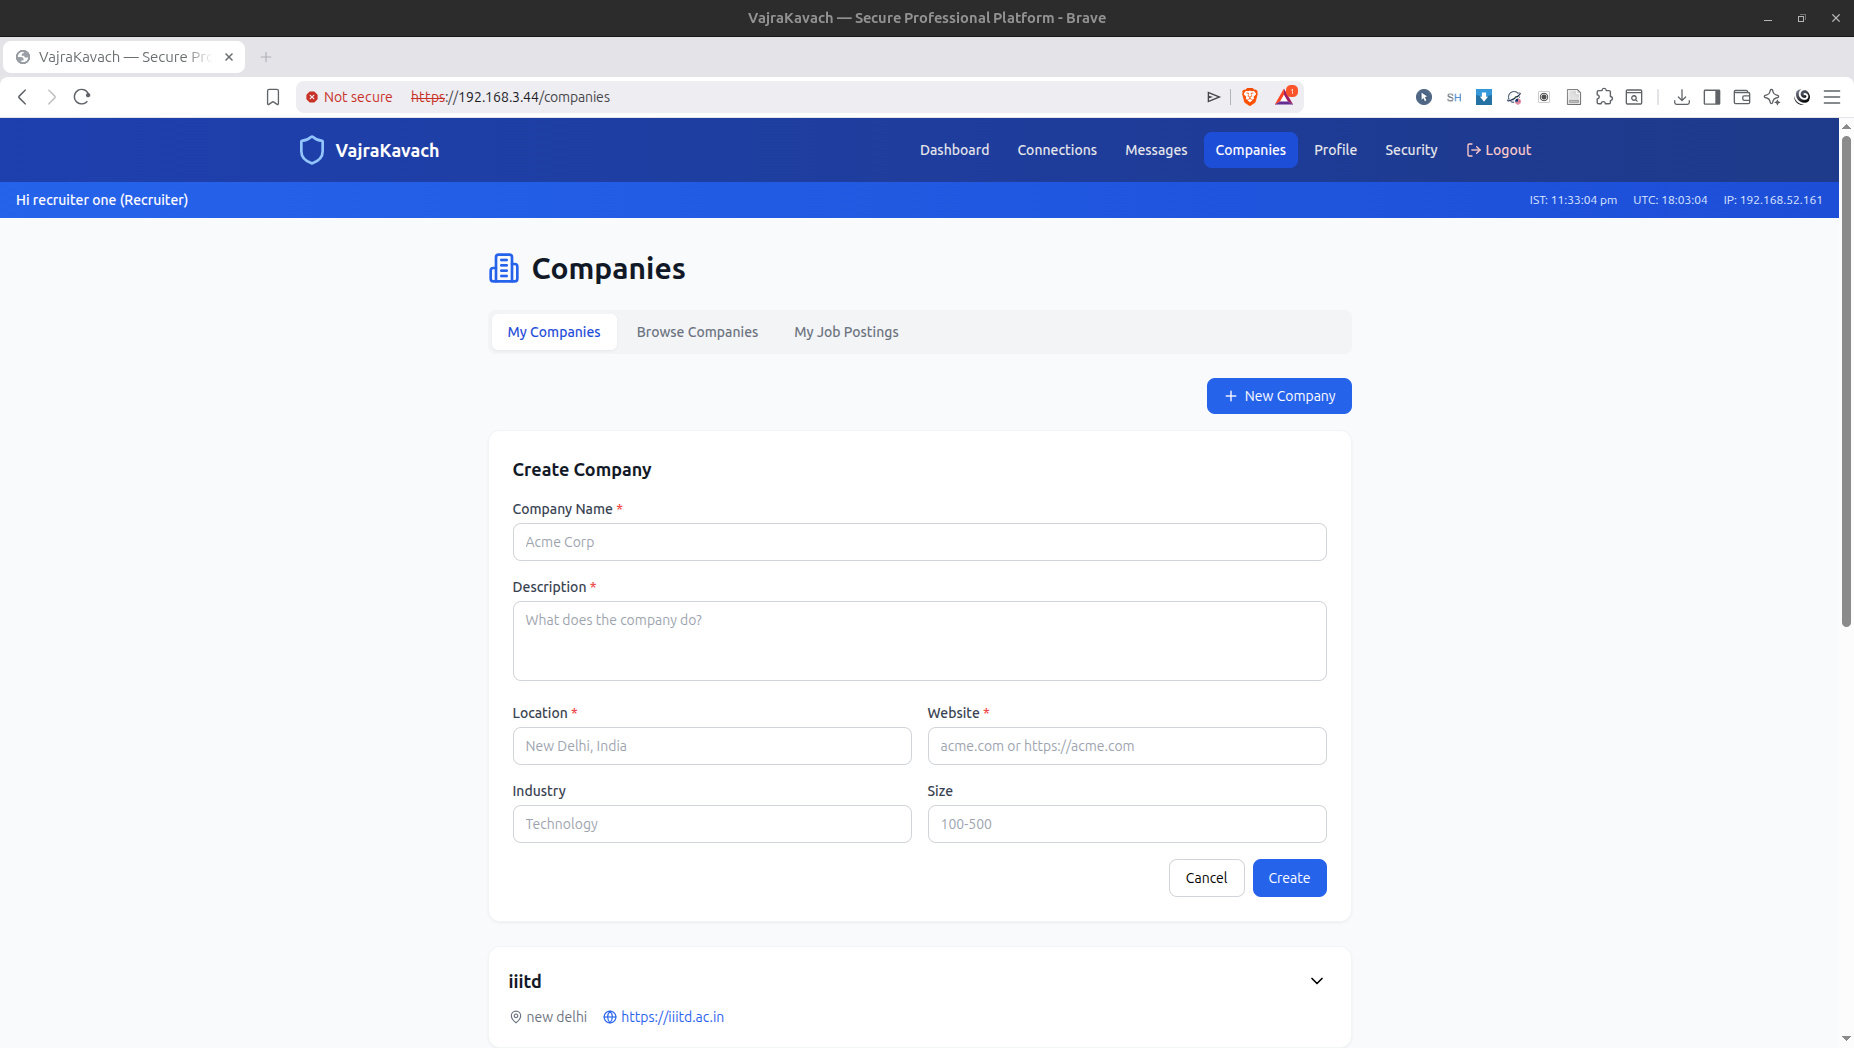
\includegraphics[width=0.85\textwidth]{screenshots/m3_company_create.png}
\caption{Company page creation form for recruiters}
\end{figure}

\begin{figure}[H]
\centering
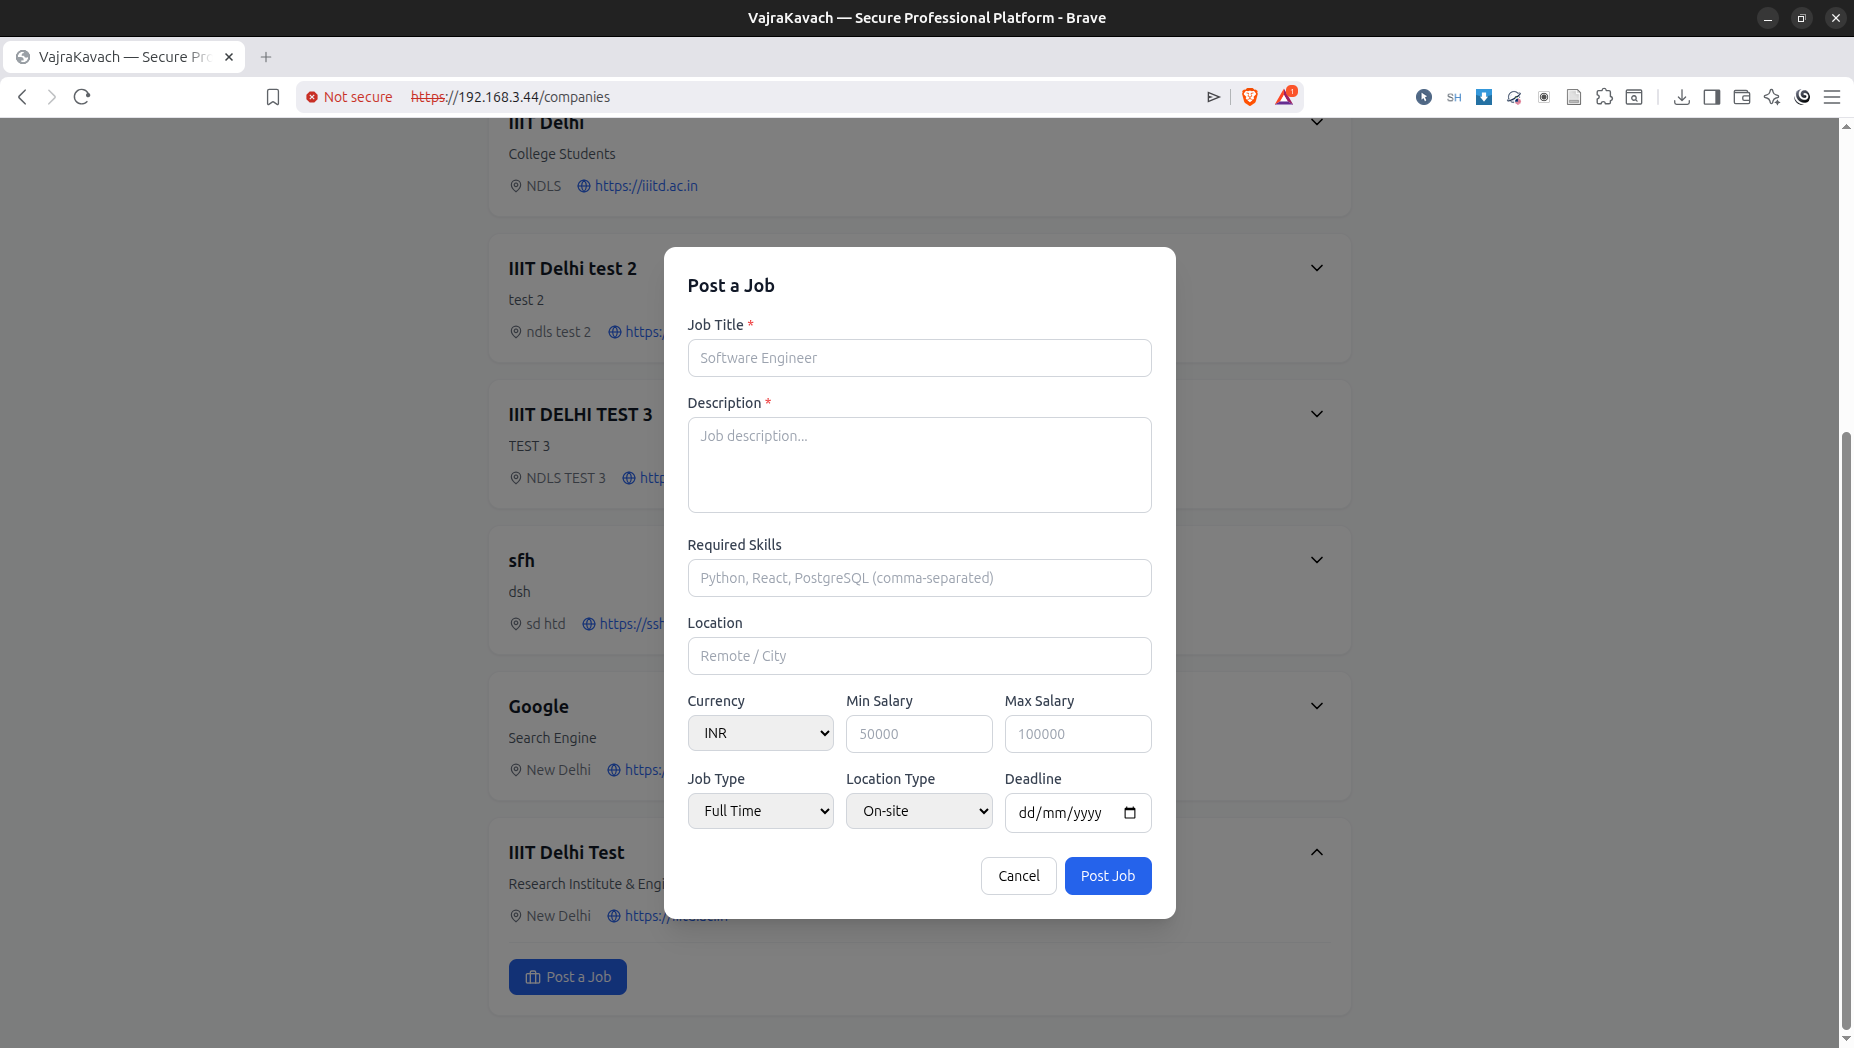
\includegraphics[width=0.85\textwidth]{screenshots/m3_job_posting.png}
\caption{Job posting form with title, description, skills, location type, and salary range}
\end{figure}

\begin{figure}[H]
\centering
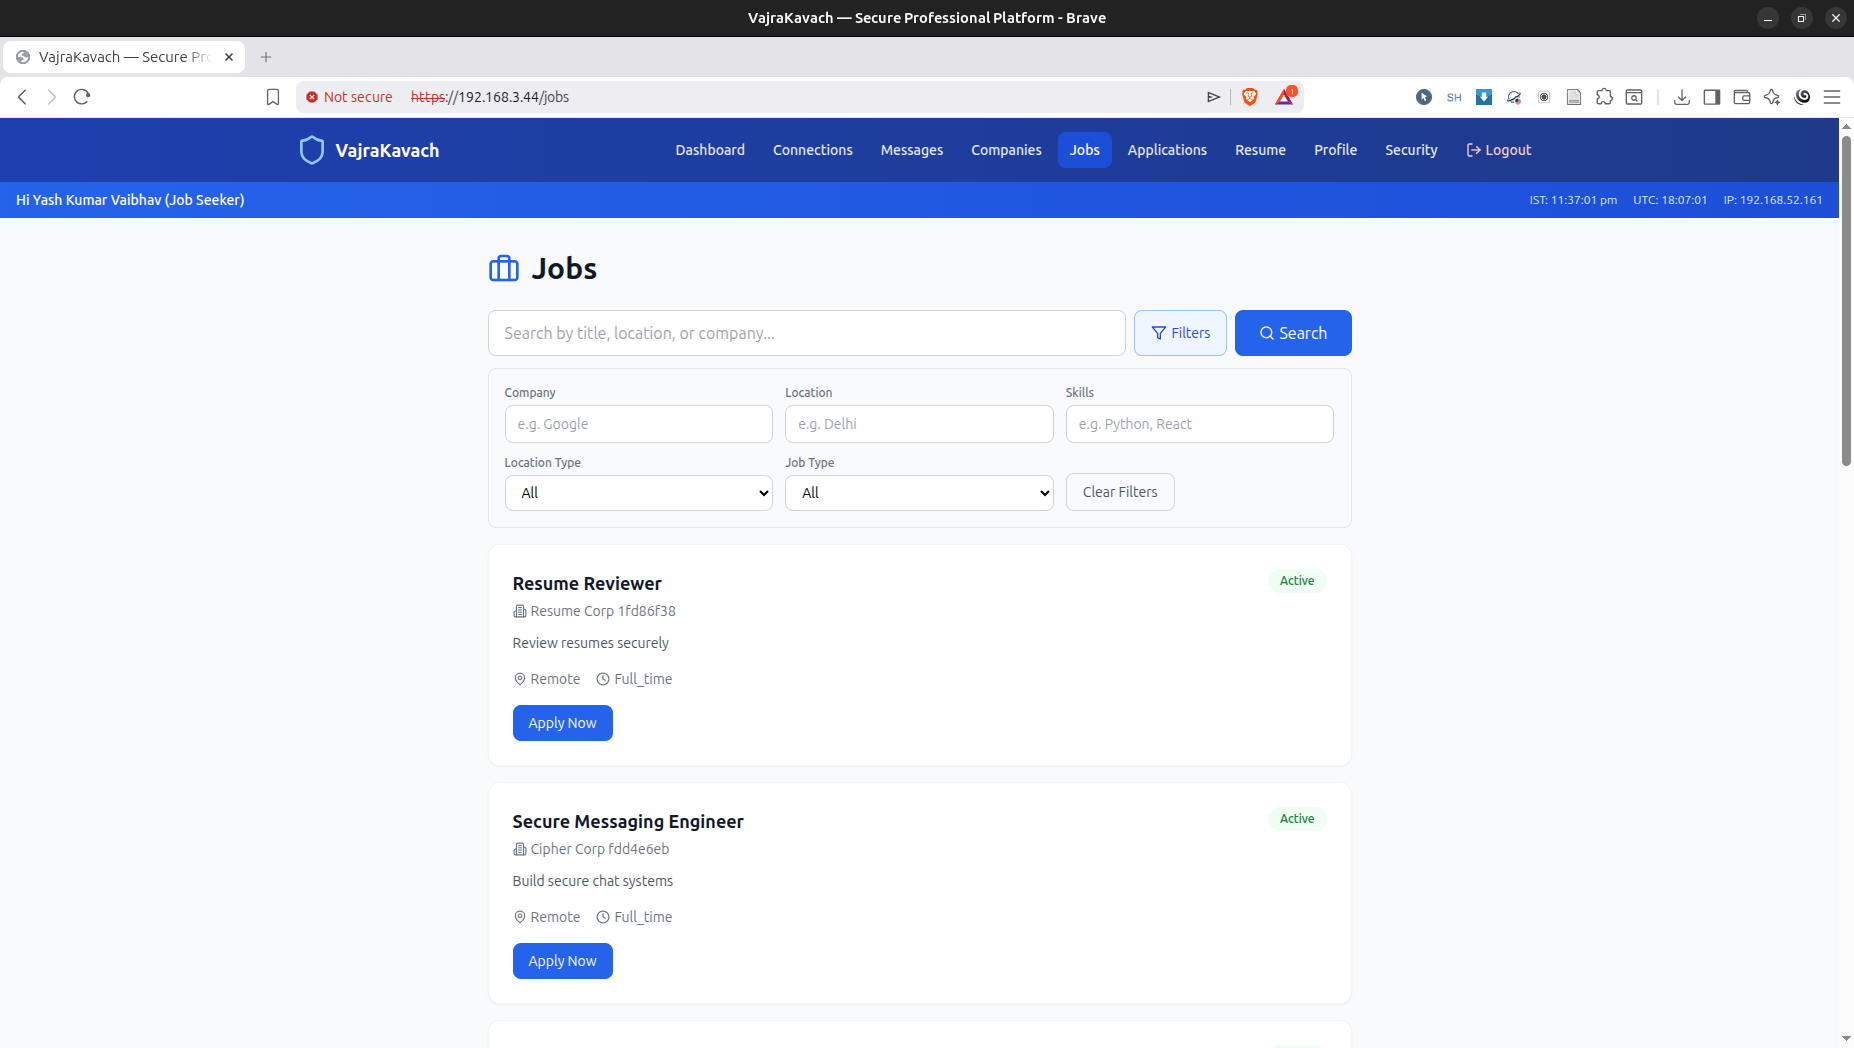
\includegraphics[width=0.85\textwidth]{screenshots/m3_job_search.png}
\caption{Job search page with keyword, location, job type, and skill filters}
\end{figure}

\newpage

% ============================================================
\section{Job Search and Application Workflow}
% ============================================================

\subsection{Overview}
Job seekers can search for jobs using advanced filters, view job details, and submit applications with an optional resume and cover note. The application system prevents duplicate submissions and enforces role-based access.

\subsection{Advanced Job Search}
The search system supports multiple simultaneous filters:
\begin{itemize}
  \item \textbf{Keyword search:} Matches against job title and description.
  \item \textbf{Company filter:} Filter by company name.
  \item \textbf{Location filter:} Case-insensitive location matching.
  \item \textbf{Location type:} Remote, On-site, or Hybrid.
  \item \textbf{Job type:} Full-time, Part-time, Internship, Contract.
  \item \textbf{Skills filter:} Comma-separated skill tags with case-insensitive substring matching.
  \item \textbf{Pagination:} Default page size of 20, maximum 100 results per page.
\end{itemize}

\subsection{Application Workflow}
\begin{enumerate}
  \item Job seeker browses or searches available jobs.
  \item Selects a job and clicks ``Apply.''
  \item Optionally attaches a previously uploaded resume and writes a cover note.
  \item System validates no duplicate application exists for the same job.
  \item Application is created with status \texttt{APPLIED}.
  \item Recruiter reviews applications and updates status through the workflow.
\end{enumerate}

\subsection{Application Model}
\begin{table}[H]
\centering
\begin{tabular}{ll}
\toprule
\textbf{Field} & \textbf{Description} \\
\midrule
\texttt{id} & UUID primary key \\
\texttt{job\_id} & Foreign key to the job listing \\
\texttt{user\_id} & Foreign key to the applicant \\
\texttt{resume\_id} & Optional link to an encrypted resume \\
\texttt{cover\_note} & Optional cover letter text \\
\texttt{status} & Enum: applied, reviewed, interviewed, rejected, offer \\
\texttt{recruiter\_notes} & Private notes from the recruiter \\
\texttt{created\_at} & Submission timestamp \\
\bottomrule
\end{tabular}
\caption{Application Data Model}
\end{table}

\subsection{Security Measures}
\begin{itemize}
  \item \textbf{Duplicate Prevention:} Server rejects multiple applications to the same job from the same user.
  \item \textbf{Authorization:} Only the applicant can withdraw; only the recruiter or admin can update status.
  \item \textbf{Audit Trail:} Every application submission and status change is logged.
\end{itemize}

\subsection{Screenshots}

\begin{figure}[H]
\centering
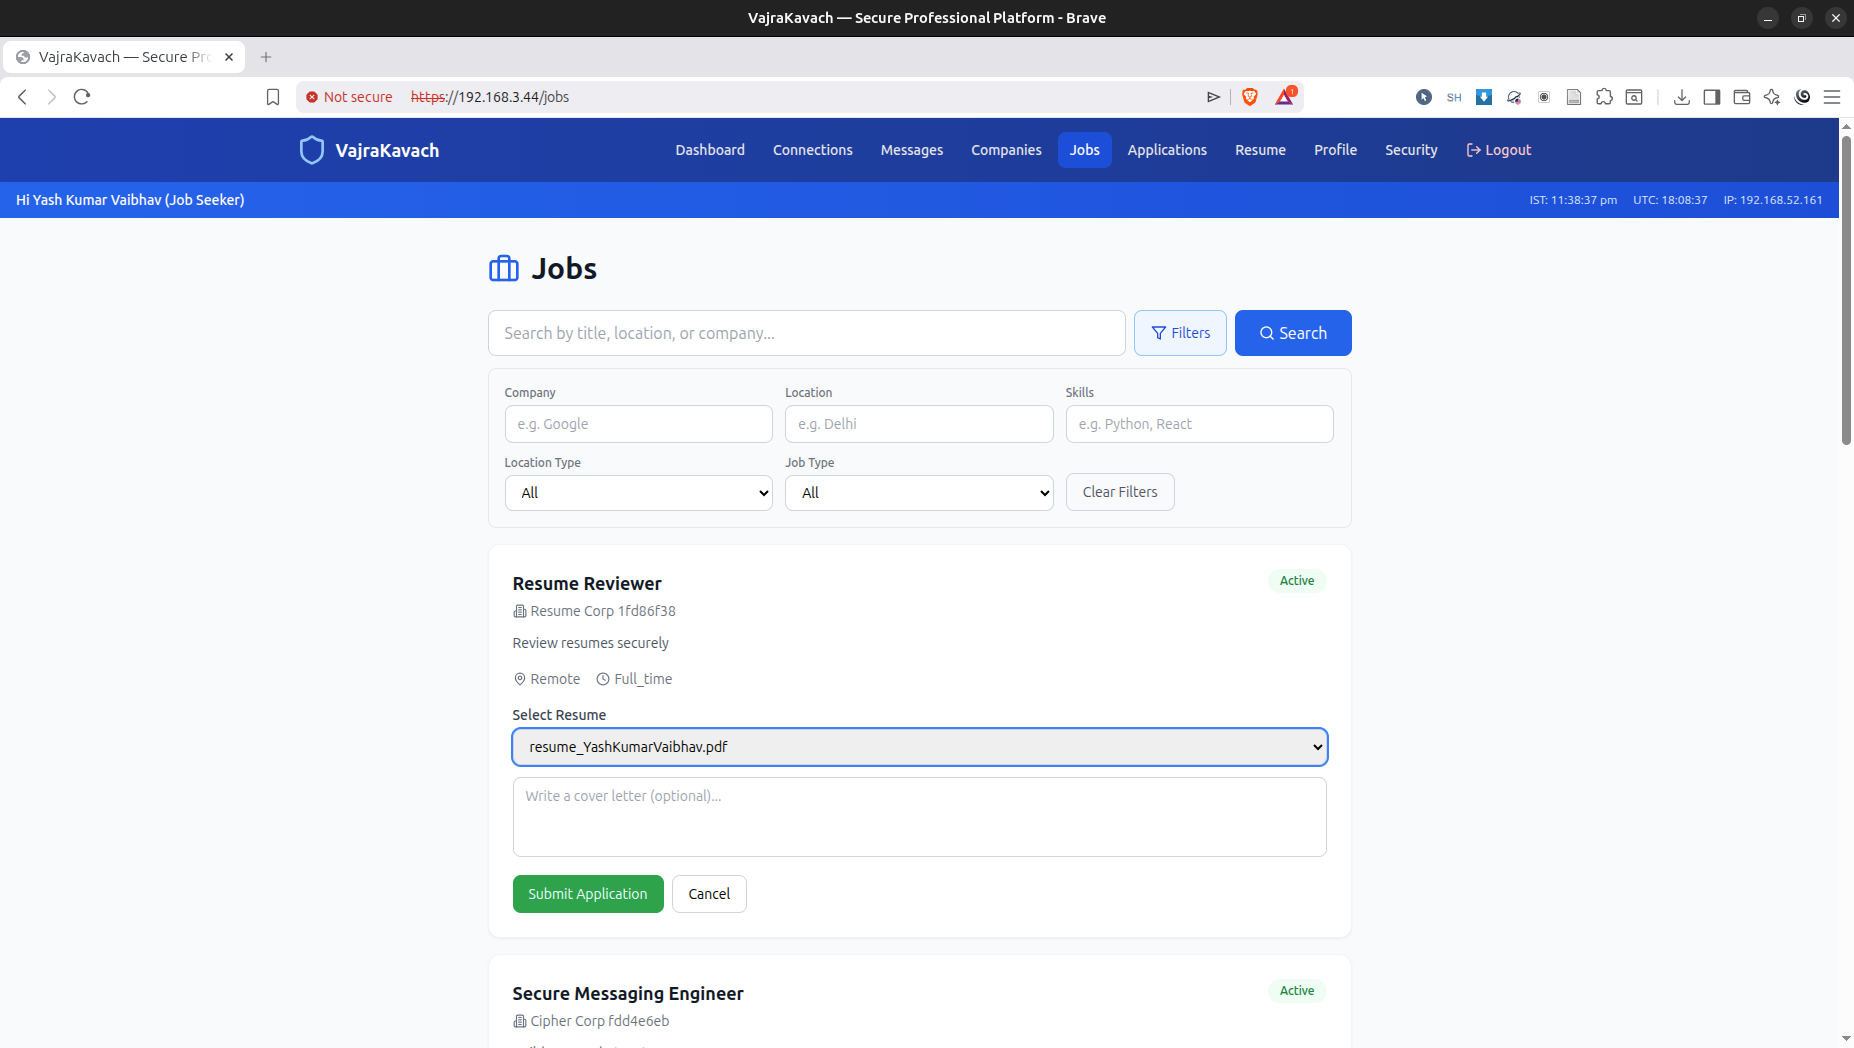
\includegraphics[width=0.85\textwidth]{screenshots/m3_apply_job.png}
\caption{Job application form with resume selection and cover note}
\end{figure}

\newpage

% ============================================================
\section{Application Status Tracking}
% ============================================================

\subsection{Overview}
Applications follow a defined lifecycle managed by recruiters. Both applicants and recruiters have dedicated views to track application progress.

\subsection{Status Workflow}
\begin{enumerate}
  \item \textbf{Applied} --- Initial state when a job seeker submits an application.
  \item \textbf{Reviewed} --- Recruiter has reviewed the application.
  \item \textbf{Interviewed} --- Candidate has been scheduled or completed an interview.
  \item \textbf{Offer} --- Job offer has been extended to the candidate.
  \item \textbf{Rejected} --- Application has been declined.
\end{enumerate}

\subsection{Recruiter Features}
\begin{itemize}
  \item View all applications for a specific job with applicant details.
  \item Update application status through the defined workflow states.
  \item Add private recruiter notes during status updates.
  \item View applicant profiles and download resumes (TOTP-gated).
\end{itemize}

\subsection{Applicant Features}
\begin{itemize}
  \item View all submitted applications with current status.
  \item Color-coded status badges for quick visual identification.
  \item Withdraw pending applications before review.
  \item View job and company details for each application.
\end{itemize}

\subsection{Audit Trail}
Each status update creates an audit log entry containing:
\begin{lstlisting}
{
  "action": "application.status_update",
  "resource": "application",
  "details": {
    "old_status": "applied",
    "new_status": "reviewed"
  },
  "ip_address": "<client_ip>"
}
\end{lstlisting}

\subsection{Screenshots}

\begin{figure}[H]
\centering
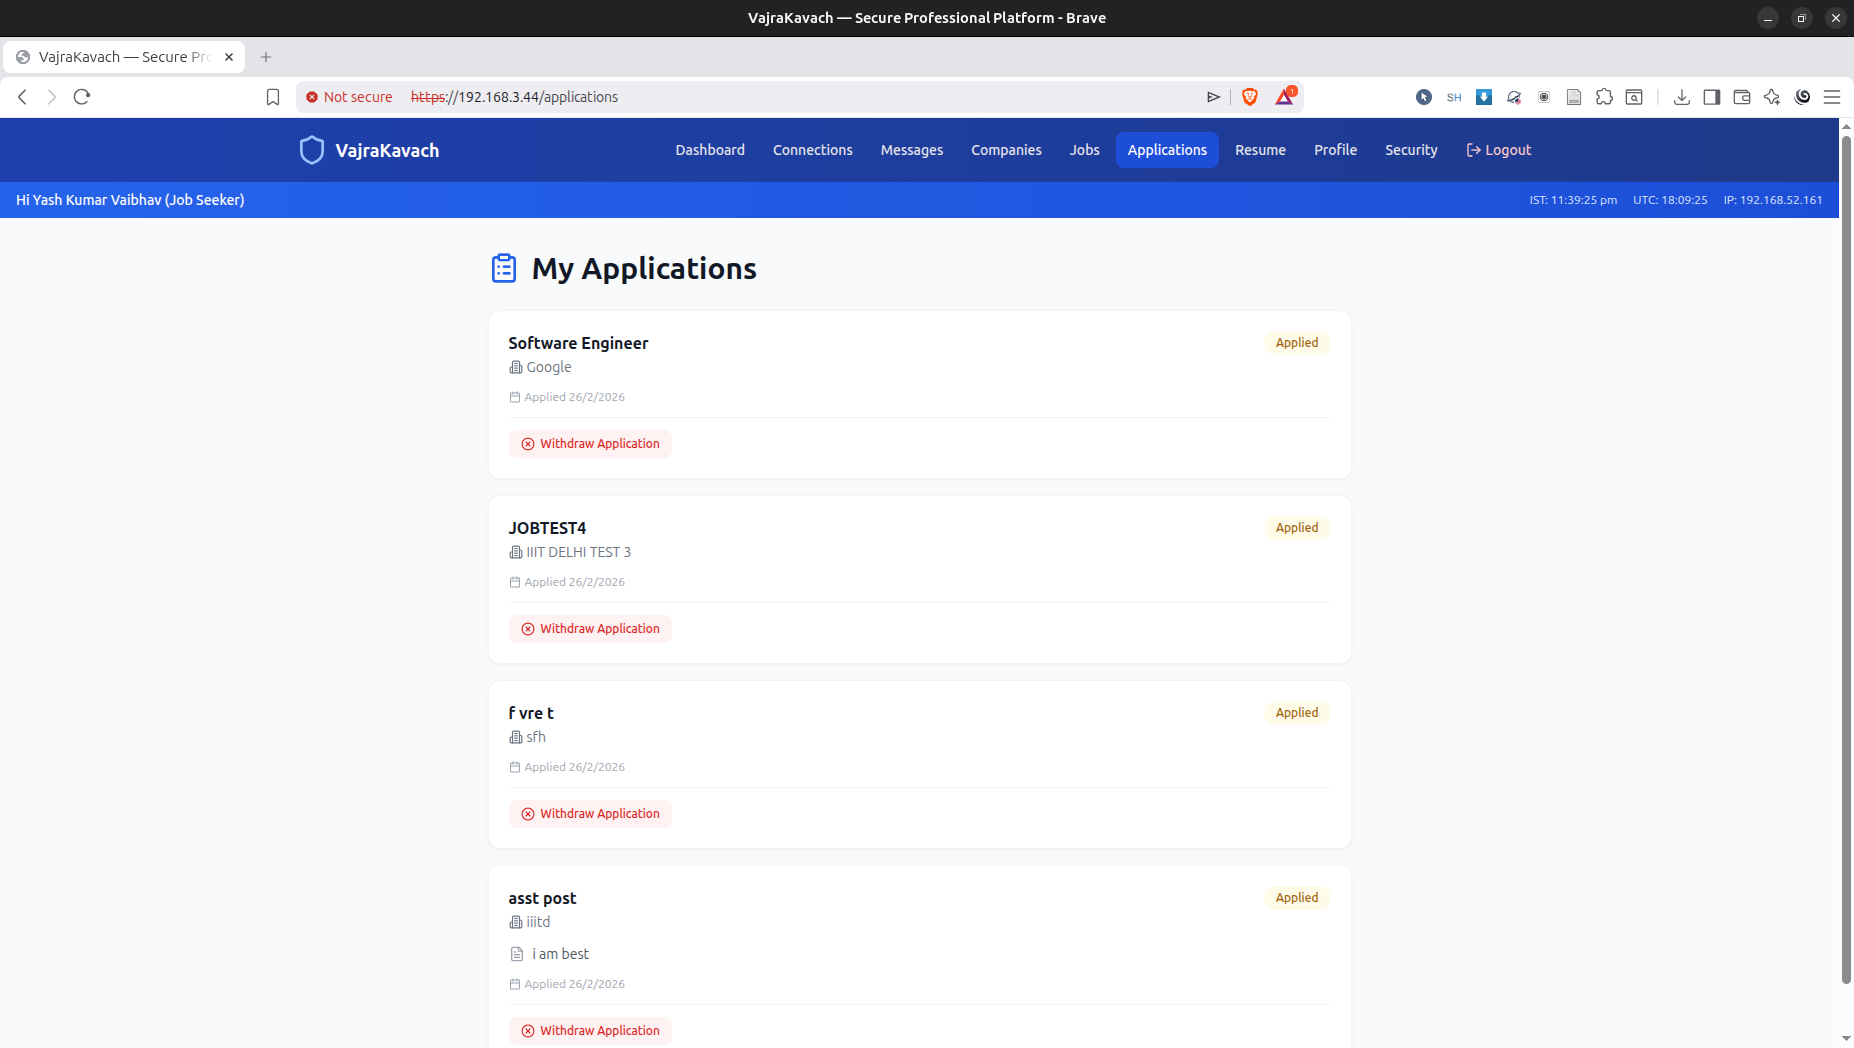
\includegraphics[width=0.85\textwidth]{screenshots/m3_application_tracking.png}
\caption{Applicant's view showing application status with color-coded badges}
\end{figure}

\begin{figure}[H]
\centering
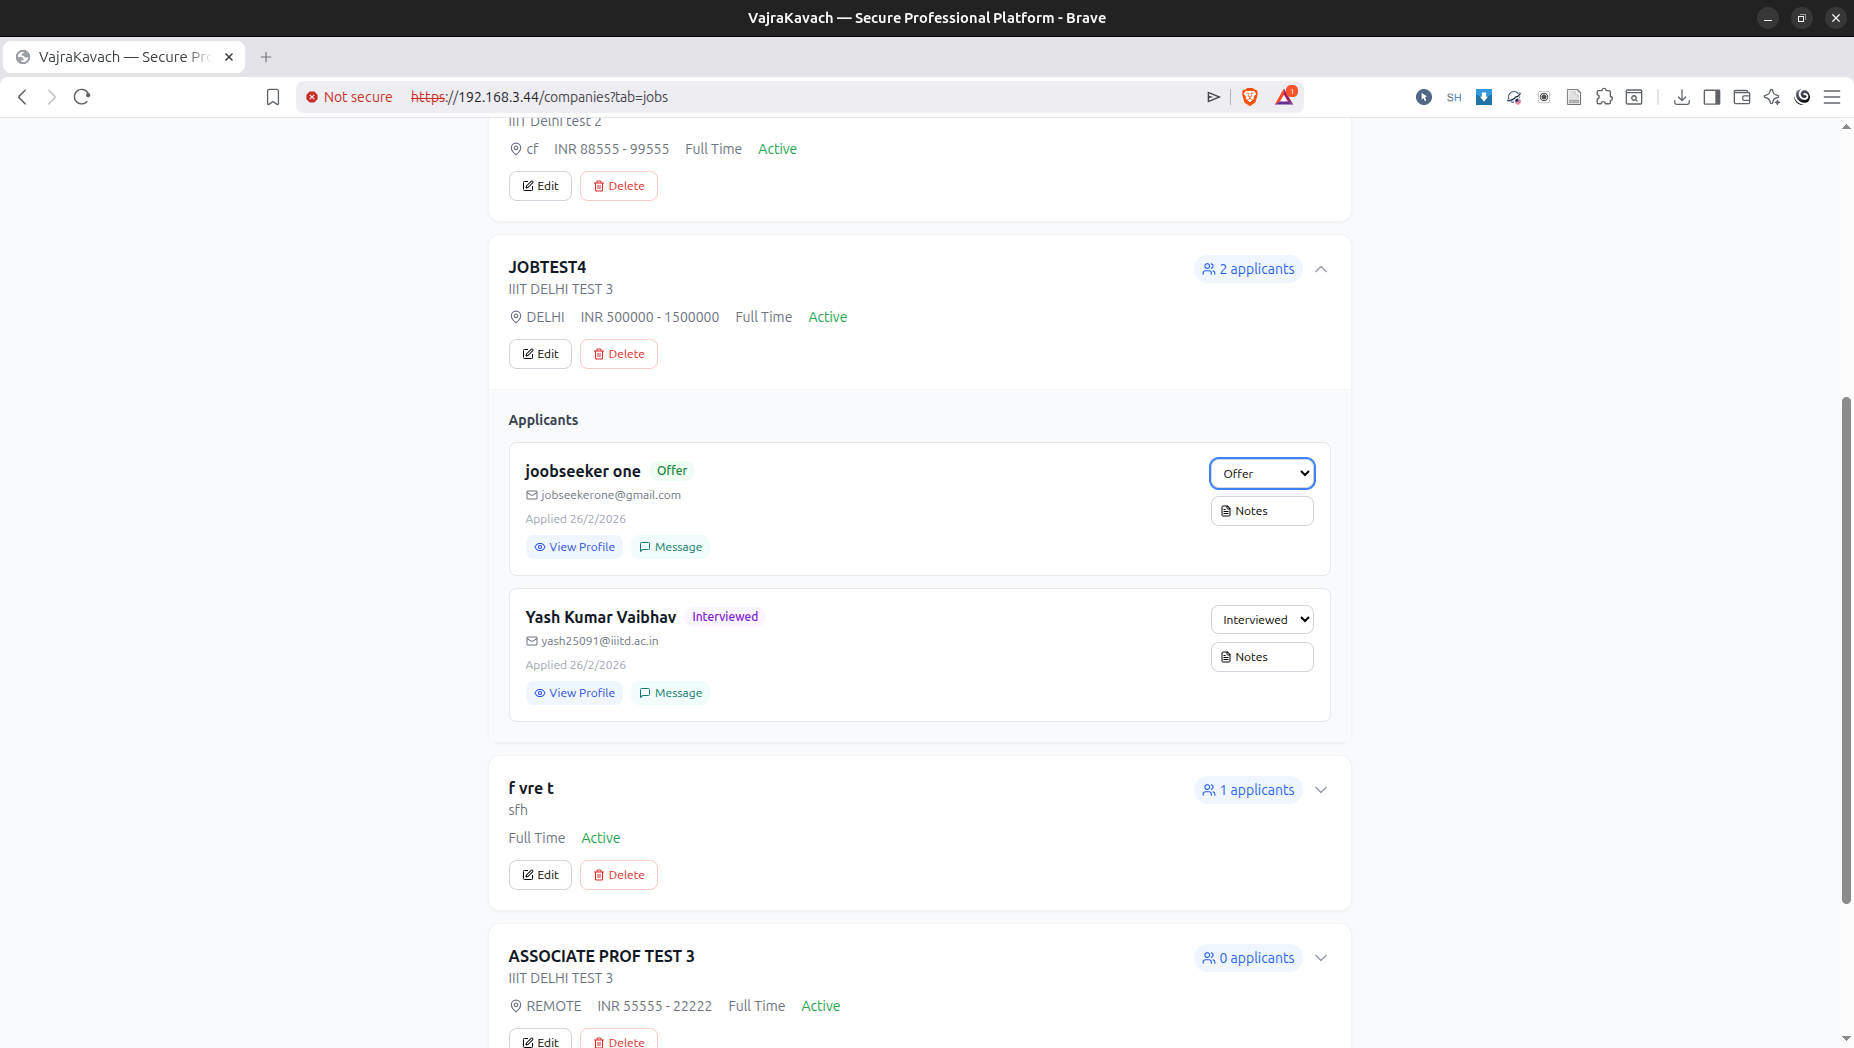
\includegraphics[width=0.85\textwidth]{screenshots/m3_recruiter_applications.png}
\caption{Recruiter's view of applications for a job with status update controls}
\end{figure}

\newpage

% ============================================================
\section{Encrypted One-to-One and Group Messaging}
% ============================================================

\subsection{Overview}
VajraKavach implements a zero-knowledge messaging system where the server stores \textbf{only ciphertext}. All message encryption and decryption happens client-side using the Web Crypto API. The system supports both one-to-one and group conversations with end-to-end encryption (E2EE).

\subsection{Encryption Architecture}
The messaging system uses a \textbf{hybrid encryption} scheme combining RSA and AES:

\begin{enumerate}
  \item A random \textbf{AES-256} session key is generated for each message.
  \item The message plaintext is encrypted with \textbf{AES-GCM} (256-bit key, 12-byte IV, 128-bit auth tag).
  \item The AES session key is encrypted with the recipient's \textbf{RSA-OAEP} public key (2048-bit).
  \item The encrypted payload is assembled as:
\end{enumerate}

\begin{lstlisting}
[2-byte key_length][RSA-encrypted AES key][12-byte IV][AES-GCM ciphertext + tag]
\end{lstlisting}

The entire payload is Base64-encoded for transmission and storage.

\subsection{One-to-One Messaging}
For direct messages, the sender encrypts the message twice --- once with the recipient's public key and once with their own --- so both parties can decrypt:

\begin{lstlisting}
E2E:{"s":"<encrypted_for_sender>","r":"<encrypted_for_recipient>"}
\end{lstlisting}

\subsection{Group Messaging}
For group conversations, each member receives an individually encrypted copy of the AES session key:

\begin{lstlisting}
E2EG:{"<user_id_1>":"<encrypted_blob>",
      "<user_id_2>":"<encrypted_blob>", ...}
\end{lstlisting}

Each participant's blob contains the AES key encrypted with their RSA public key, ensuring only group members can decrypt.

\subsection{Client-Side Key Management}
\begin{itemize}
  \item RSA-2048 key pairs are generated during user registration.
  \item Public keys are stored on the server for key exchange.
  \item Private keys are encrypted with \textbf{PBKDF2} (250,000 iterations, SHA-256) derived from the user's password and stored locally in \textbf{IndexedDB}.
  \item During a session, the decrypted private key is held in \texttt{sessionStorage} and cleared on tab close.
\end{itemize}

\subsection{Server-Side Validation}
The backend enforces that only encrypted messages are accepted:
\begin{itemize}
  \item Rejects any message not prefixed with \texttt{E2E:} or \texttt{E2EG:}.
  \item Validates the JSON structure of the encrypted payload.
  \item Verifies the Base64-encoded ciphertext contains a valid RSA-OAEP + AES-GCM hybrid structure.
  \item \textbf{Never stores or processes plaintext message content.}
\end{itemize}

\subsection{Group Management}
\begin{itemize}
  \item Any authenticated user can create a group conversation with selected members.
  \item Existing members can add new members to the group.
  \item The group creator or the member themselves can remove members.
  \item Group membership changes are validated server-side.
\end{itemize}

\subsection{Security Summary}
\begin{table}[H]
\centering
\begin{tabular}{ll}
\toprule
\textbf{Property} & \textbf{Implementation} \\
\midrule
Confidentiality & RSA-OAEP (2048-bit) + AES-256-GCM hybrid encryption \\
Integrity & AES-GCM 128-bit authentication tag \\
Zero Knowledge & Server stores only ciphertext; no plaintext access \\
Key Exchange & RSA public keys exchanged via authenticated API \\
Key Storage & PBKDF2-encrypted private keys in IndexedDB \\
Forward Secrecy & Per-message random AES session keys \\
\bottomrule
\end{tabular}
\caption{E2EE Security Properties}
\end{table}

\subsection{Screenshots}

\begin{figure}[H]
\centering
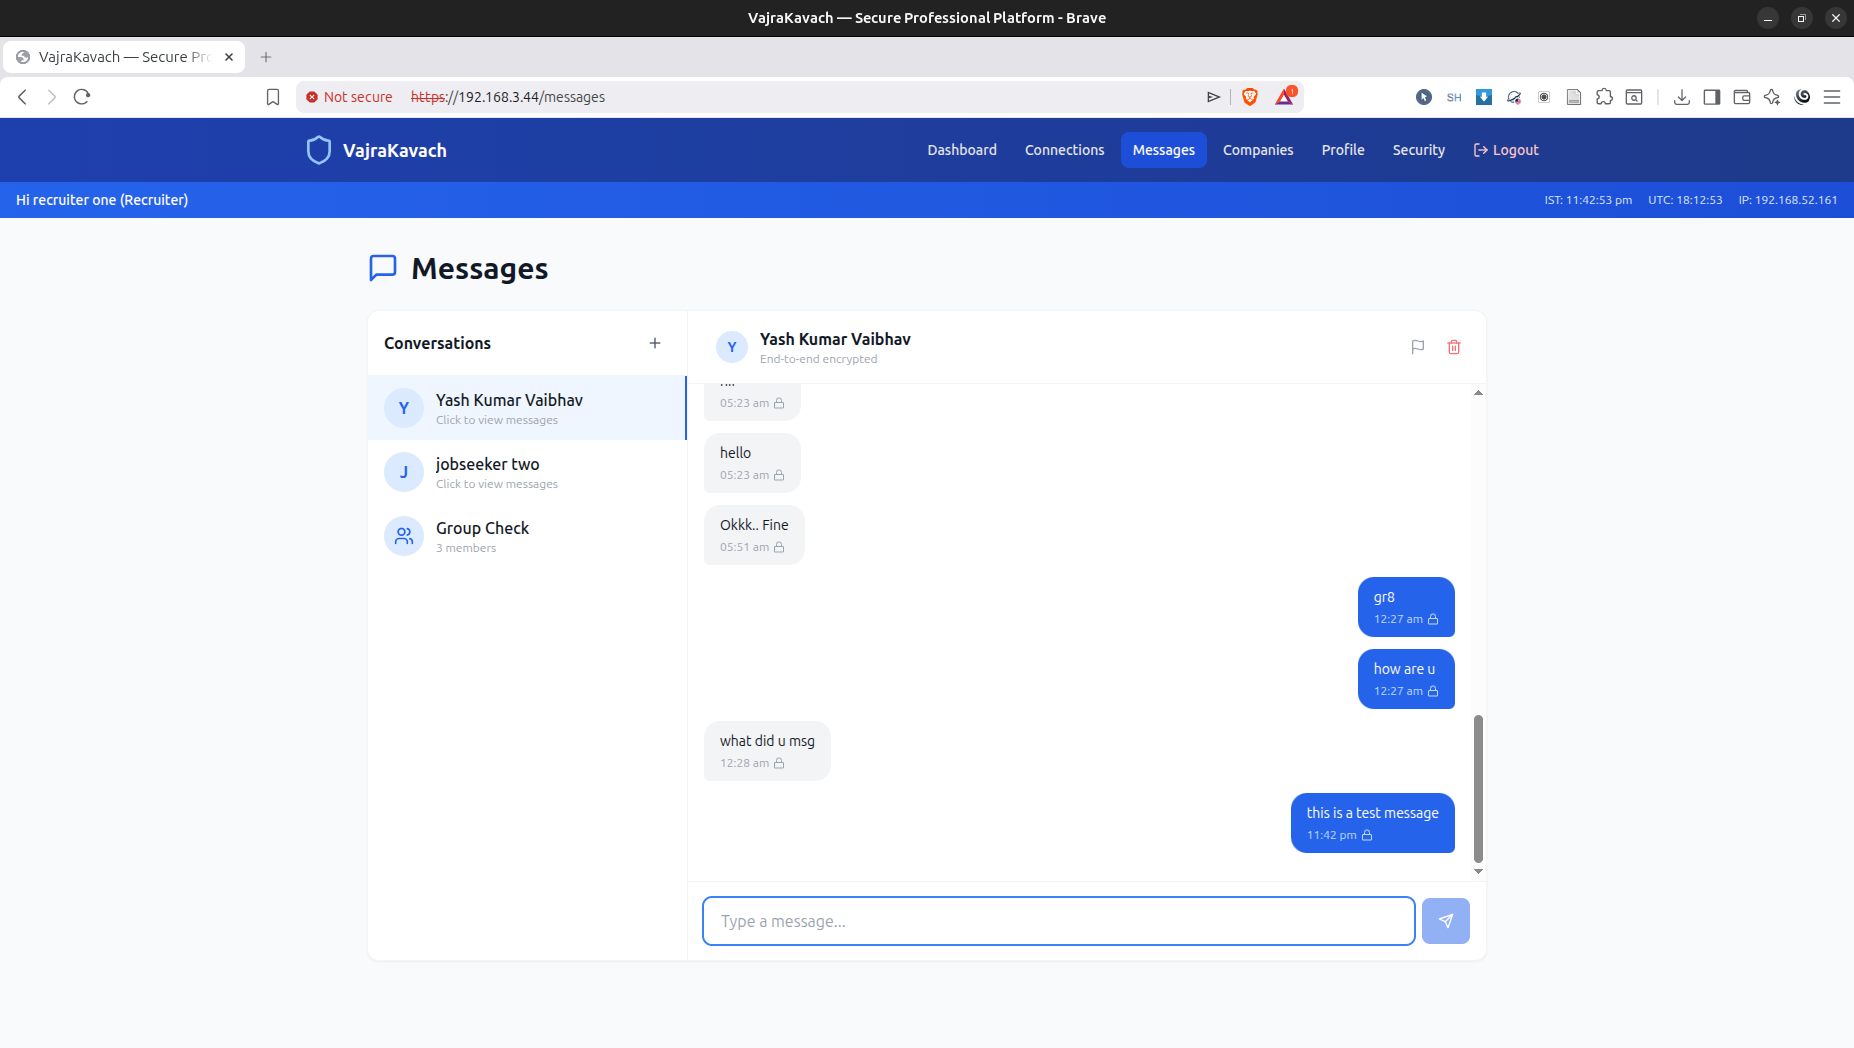
\includegraphics[width=0.85\textwidth]{screenshots/m3_messaging_conversation.png}
\caption{One-to-one encrypted conversation showing lock icon and decrypted messages}
\end{figure}

\begin{figure}[H]
\centering
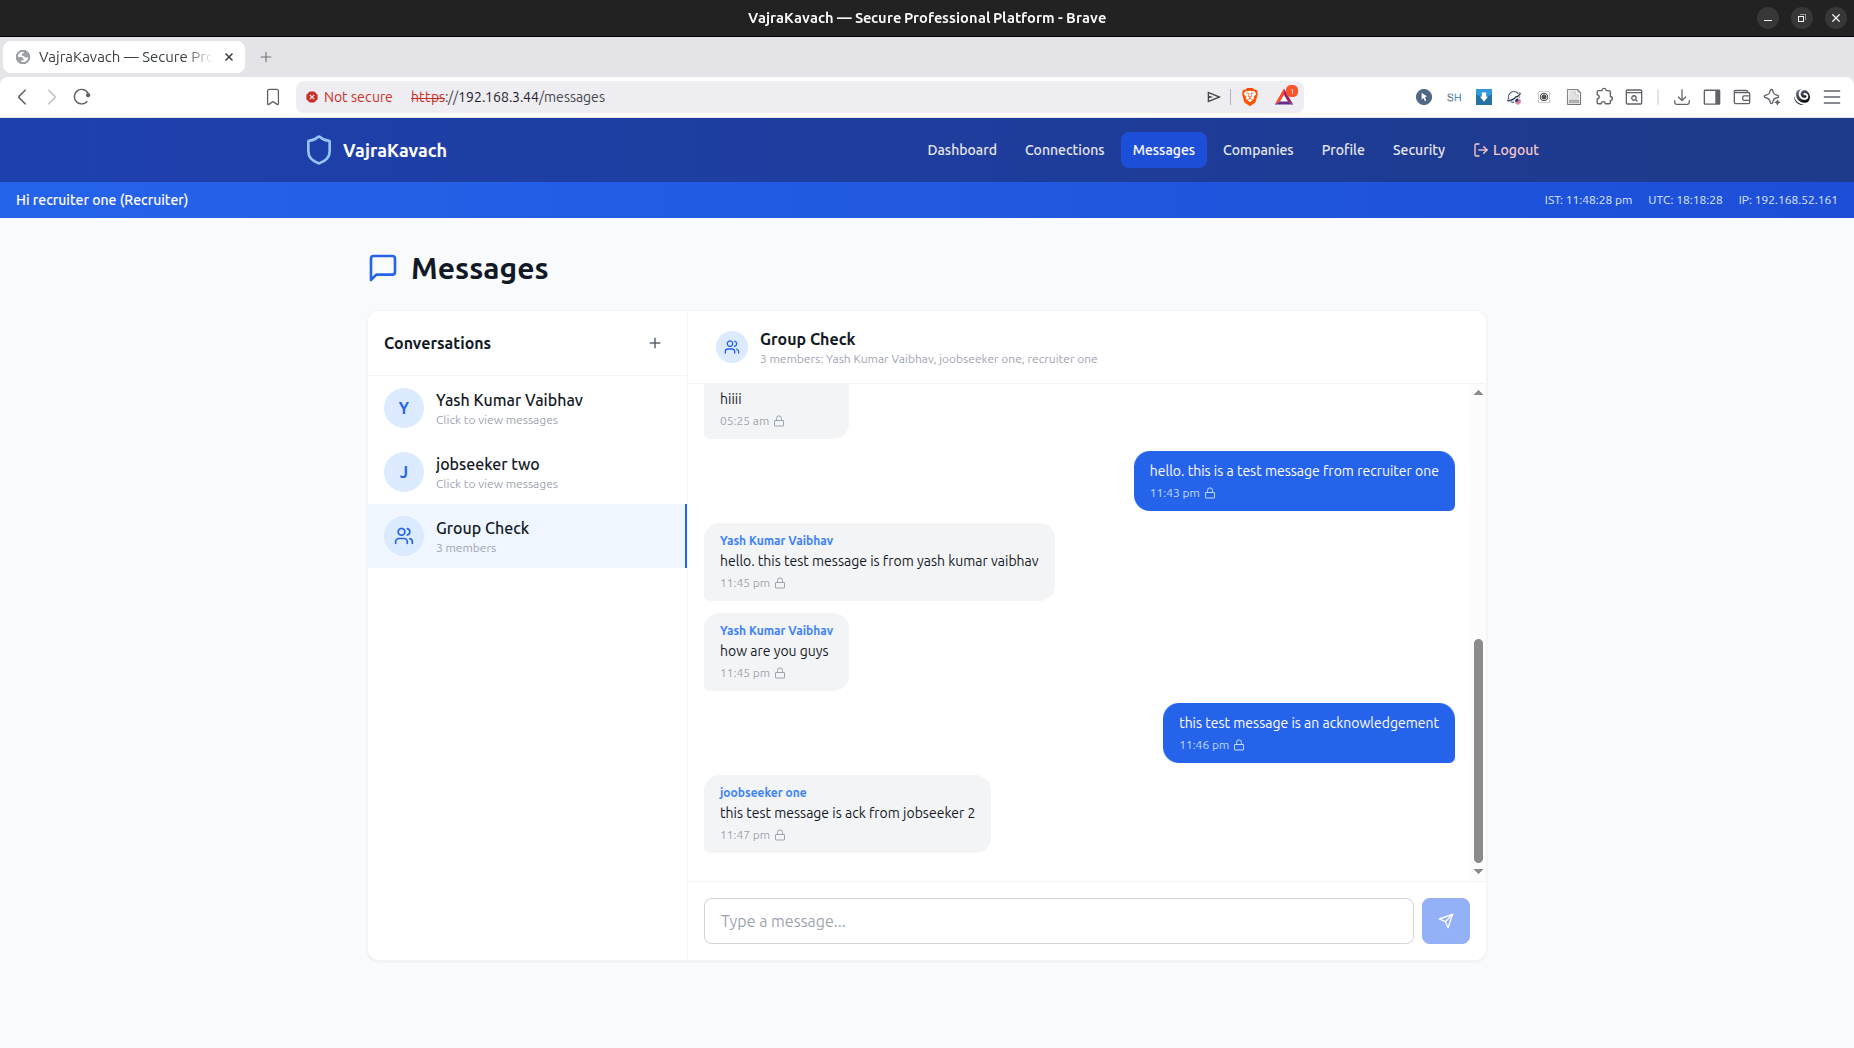
\includegraphics[width=0.85\textwidth]{screenshots/m3_messaging_group.png}
\caption{Group messaging with multiple participants and E2EE indicator}
\end{figure}

\begin{figure}[H]
\centering
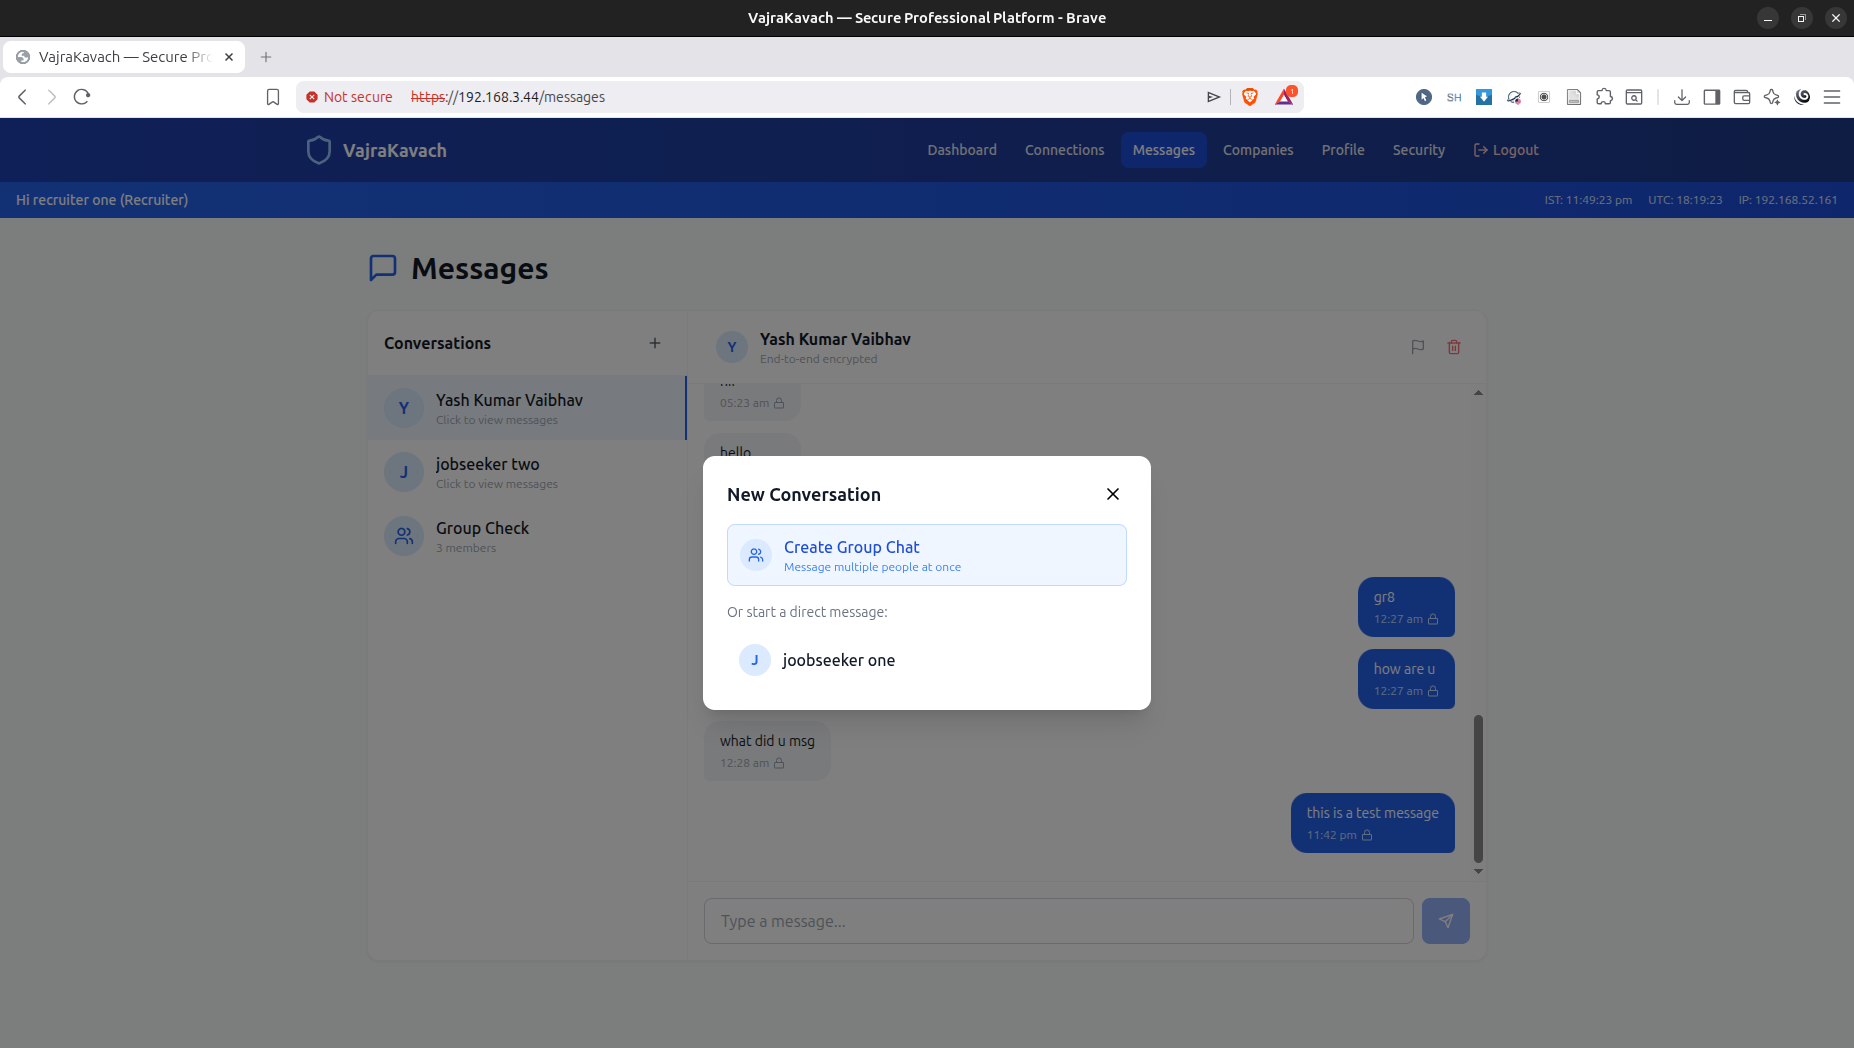
\includegraphics[width=0.85\textwidth]{screenshots/m3_messaging_conversations_list.png}
\caption{Conversations list showing one-to-one and group chats}
\end{figure}

\newpage

% ============================================================
\section{Server-Side Encrypted Announcements}
% ============================================================

\subsection{Overview}
Platform admins can broadcast announcements to all users. Announcements use server-side encryption with \textbf{Fernet (AES-128-CBC + HMAC-SHA256)} for at-rest protection, distinct from E2EE messaging.

\subsection{Announcement Flow}
\begin{enumerate}
  \item Platform admin composes an announcement with title and content.
  \item Both title and content are encrypted server-side using Fernet before storage.
  \item All authenticated users can retrieve announcements; the server decrypts on-the-fly.
  \item Announcements support soft-delete via an \texttt{is\_active} flag.
\end{enumerate}

\subsection{Security Measures}
\begin{itemize}
  \item Only platform admins can create or delete announcements.
  \item Encryption key is stored in environment configuration, never in source code.
  \item Decryption errors are handled gracefully without exposing internals.
\end{itemize}

\newpage

% ============================================================
\section{Initial Admin Logging}
% ============================================================

\subsection{Overview}
VajraKavach implements a two-tier tamper-evident logging system: \textbf{hash-chained audit logs} and a \textbf{blockchain layer} with proof-of-work. All critical platform actions are recorded and verifiable.

\subsection{Hash-Chained Audit Logs}
Every critical action on the platform generates an audit log entry with the following structure:

\begin{table}[H]
\centering
\begin{tabular}{ll}
\toprule
\textbf{Field} & \textbf{Description} \\
\midrule
\texttt{action} & Action identifier (e.g., \texttt{user.login}, \texttt{job.create}) \\
\texttt{resource} & Affected entity type (user, job, application, etc.) \\
\texttt{resource\_id} & UUID of the affected entity \\
\texttt{details} & JSON with contextual information \\
\texttt{ip\_address} & Client IP address (supports IPv6) \\
\texttt{entry\_hash} & SHA-256 hash of this entry + previous hash \\
\texttt{previous\_hash} & SHA-256 hash of the preceding entry \\
\bottomrule
\end{tabular}
\caption{Audit Log Entry Structure}
\end{table}

\textbf{Hash Chain Construction:}
\begin{lstlisting}
entry_hash = SHA-256(
  previous_hash | action | user_id | resource |
  resource_id | details | ip_address | timestamp
)
\end{lstlisting}

The first entry uses a genesis hash of 64 zeros. Modifying any entry breaks all subsequent hashes in the chain.

\subsection{Logged Actions}
The following categories of actions are logged:
\begin{itemize}
  \item \textbf{Authentication:} Login, registration, password changes.
  \item \textbf{Companies:} Create, update, delete operations.
  \item \textbf{Jobs:} Create, update, delete, delist operations.
  \item \textbf{Applications:} Submissions and all status transitions.
  \item \textbf{Messages:} Send events (content not logged --- only metadata).
  \item \textbf{Admin Actions:} User suspensions, promotions, deletions.
  \item \textbf{Blockchain:} Block mining operations.
\end{itemize}

\subsection{Blockchain Layer}
Audit log entries are periodically aggregated into blockchain blocks with proof-of-work:

\begin{table}[H]
\centering
\begin{tabular}{ll}
\toprule
\textbf{Field} & \textbf{Description} \\
\midrule
\texttt{block\_number} & Sequential block index \\
\texttt{previous\_block\_hash} & SHA-256 of the previous block \\
\texttt{merkle\_root} & Merkle tree root of constituent entry hashes \\
\texttt{nonce} & Proof-of-work nonce \\
\texttt{block\_hash} & SHA-256 hash with 2 leading zeros (difficulty target) \\
\texttt{entry\_count} & Number of audit entries in the block \\
\texttt{entry\_ids} & Comma-separated audit log entry IDs \\
\bottomrule
\end{tabular}
\caption{Blockchain Block Structure}
\end{table}

\textbf{Merkle Tree:} Entry hashes are paired and hashed recursively until a single root remains, cryptographically committing to all entries in the block.

\textbf{Proof-of-Work:} The block hash must start with 2 leading zeros (difficulty = 2). A nonce is incremented until a valid hash is found.

\subsection{Integrity Verification}
Two verification endpoints are provided:
\begin{itemize}
  \item \textbf{Audit Log Verification} (\texttt{/api/admin/audit-logs/verify-integrity}): Recomputes each entry's hash and validates the chain linkage.
  \item \textbf{Blockchain Verification} (\texttt{/api/admin/blockchain/verify}): Validates block hashes, proof-of-work, Merkle roots, and sequential block numbering.
\end{itemize}

\subsection{Screenshots}

\begin{figure}[H]
\centering
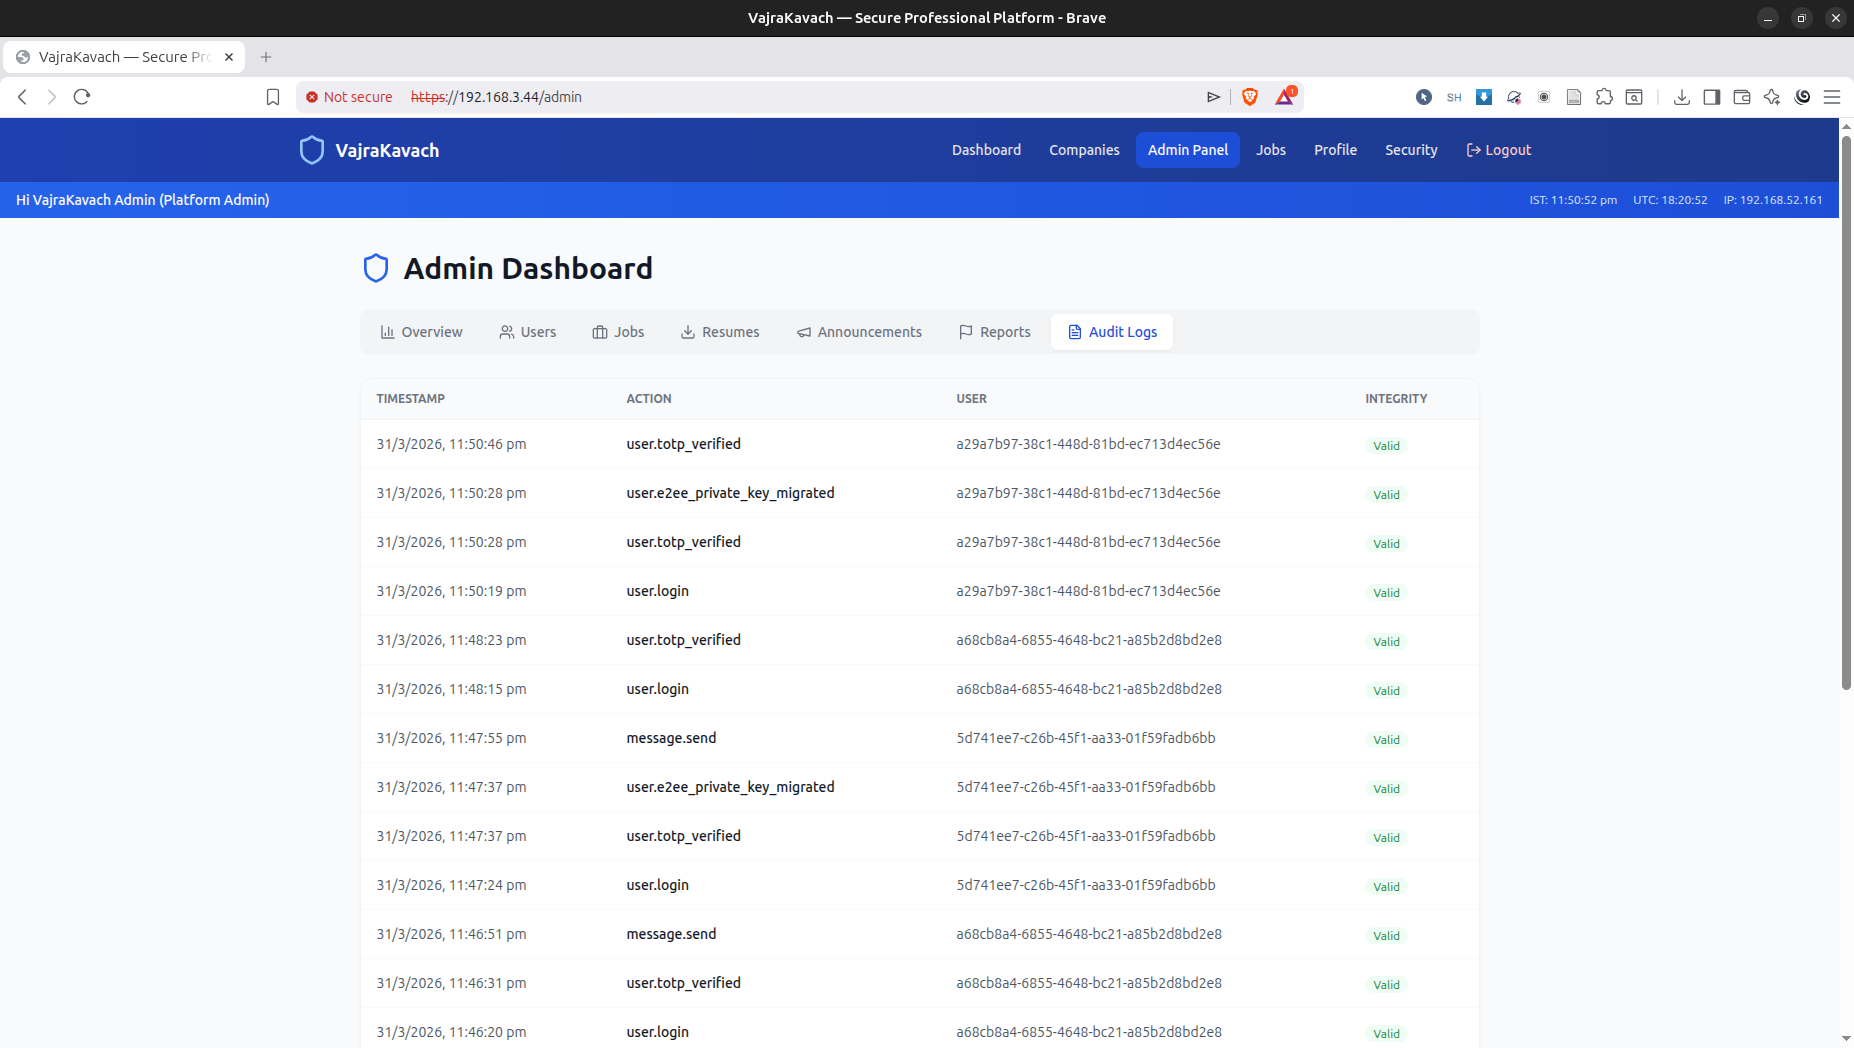
\includegraphics[width=0.85\textwidth]{screenshots/m3_audit_logs.png}
\caption{Admin audit logs view showing hash-chained entries with action details}
\end{figure}

\begin{figure}[H]
\centering
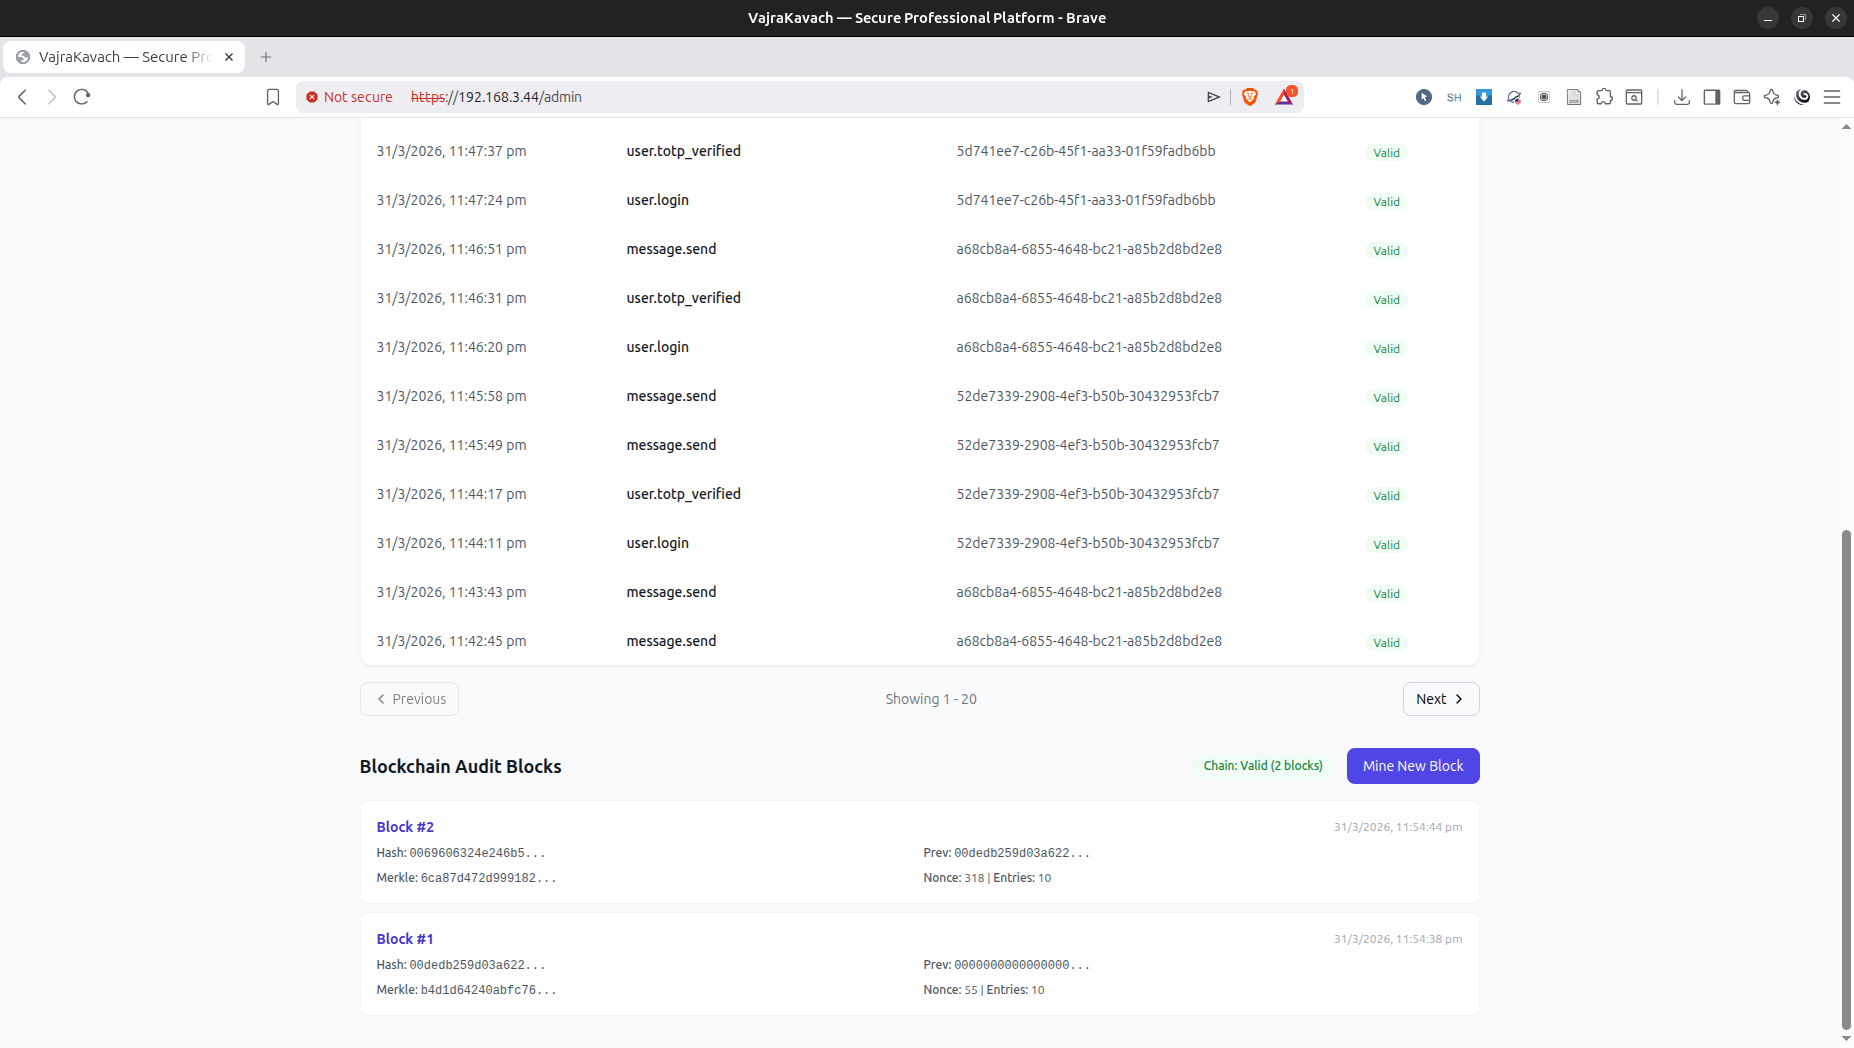
\includegraphics[width=0.85\textwidth]{screenshots/m3_blockchain_blocks.png}
\caption{Blockchain blocks view showing block hashes, Merkle roots, and entry counts}
\end{figure}

\newpage

% ============================================================
\section{Bonus Features}
% ============================================================

\subsection{Blockchain-Based Tamper-Evident Logging (+6\%)}
As described in Section~6, the platform implements a full blockchain layer on top of hash-chained audit logs. Key properties:
\begin{itemize}
  \item SHA-256 Merkle tree roots for cryptographic commitment to block contents.
  \item Proof-of-work mining with configurable difficulty.
  \item End-to-end verification of blockchain integrity.
  \item Genesis block with deterministic initial hash.
\end{itemize}

\subsection{Resume Parsing and Intelligent Matching (+2\%)}
The platform includes automated resume parsing and job--candidate match scoring:
\begin{itemize}
  \item \textbf{PDF Parsing:} Uploaded resumes are parsed server-side to extract text and identify skills using pattern matching and NLP techniques.
  \item \textbf{Skill Extraction:} Detected skills are stored alongside the resume for quick matching.
  \item \textbf{Match Scoring:} When a candidate applies to a job, the system computes a match score by comparing extracted resume skills against the job's required skills.
  \item \textbf{Recruiter View:} Match scores are displayed to recruiters in the application review interface.
\end{itemize}

\newpage

% ============================================================
\section{User Reporting System}
% ============================================================

\subsection{Overview}
Users can report other users for policy violations. Reports are reviewed by admins through the admin dashboard.

\subsection{Report Categories}
\begin{itemize}
  \item \textbf{Spam} --- Unsolicited or irrelevant content.
  \item \textbf{Harassment} --- Abusive or threatening behavior.
  \item \textbf{Fraud} --- Deceptive job postings or profiles.
  \item \textbf{Inappropriate Content} --- Violation of community guidelines.
  \item \textbf{Other} --- General policy violations.
\end{itemize}

\subsection{Admin Review Workflow}
\begin{enumerate}
  \item Reports appear in the admin dashboard under the Reports tab.
  \item Admins can review report details (reporter, reported user, category, description).
  \item Actions: Mark as Reviewed, Resolve, or Dismiss.
  \item All report actions are logged in the audit trail.
\end{enumerate}

\newpage

% ============================================================
\section{Technology Stack Compliance}
% ============================================================

\begin{table}[H]
\centering
\begin{tabular}{lll}
\toprule
\textbf{Requirement} & \textbf{Technology} & \textbf{Status} \\
\midrule
Operating System & Ubuntu (VM) & \checkmark \\
Database & PostgreSQL & \checkmark \\
Web Server & Nginx (reverse proxy + TLS) & \checkmark \\
Backend & Python (FastAPI) & \checkmark \\
Frontend & React (Vite) & \checkmark \\
Password Hashing & Argon2id (passlib) & \checkmark \\
TOTP & pyotp + qrcode & \checkmark \\
E2EE & RSA-OAEP + AES-256-GCM (Web Crypto API) & \checkmark \\
Resume Encryption & Fernet (AES-128-CBC + HMAC-SHA256) & \checkmark \\
Audit Logging & SHA-256 hash chaining & \checkmark \\
Blockchain & SHA-256 proof-of-work + Merkle trees & \checkmark \\
HTTPS/TLS & Self-signed certificates via Nginx & \checkmark \\
\bottomrule
\end{tabular}
\caption{Technology Stack Compliance Matrix}
\end{table}

\newpage

% ============================================================
\section{Summary}
% ============================================================

Milestone~3 delivers the core job platform and secure communication features of VajraKavach:

\begin{enumerate}
  \item \textbf{Company Pages \& Job Postings} --- Recruiters create company pages and post jobs with advanced attributes (location type, job type, salary range, required skills, deadlines). Role-based access control enforces ownership.

  \item \textbf{Job Search \& Application Workflow} --- Multi-filter job search (keyword, company, location, skills, job type) with pagination. Job seekers apply with optional resume and cover note; duplicate applications are prevented.

  \item \textbf{Application Status Tracking} --- Five-stage status workflow (Applied $\rightarrow$ Reviewed $\rightarrow$ Interviewed $\rightarrow$ Offer / Rejected) with recruiter notes, color-coded badges, and full audit trail of every status change.

  \item \textbf{End-to-End Encrypted Messaging} --- Zero-knowledge architecture where the server stores only ciphertext. Hybrid RSA-OAEP + AES-256-GCM encryption for both one-to-one and group conversations. Client-side key management with PBKDF2-protected private keys in IndexedDB.

  \item \textbf{Server-Side Encrypted Announcements} --- Fernet-encrypted broadcast messages from platform admins with at-rest protection.

  \item \textbf{Tamper-Evident Audit Logging} --- SHA-256 hash-chained audit logs covering all critical platform actions, with integrity verification endpoint.

  \item \textbf{Blockchain Layer (Bonus)} --- Proof-of-work blockchain with Merkle tree roots aggregating audit entries into immutable, verifiable blocks.

  \item \textbf{Resume Parsing \& Match Scoring (Bonus)} --- Automated skill extraction from uploaded PDFs with job--candidate match scoring for recruiters.
\end{enumerate}

\vspace{0.5cm}
\noindent All security measures follow best practices as outlined in the course requirements. The codebase is version-controlled and ready for the Final Evaluation (PKI integration, TOTP virtual keyboard, attack defense demonstration).

\vspace{1cm}
\noindent\textbf{Repository:} \url{https://github.com/yashkumarvaibhav/VajraKavach}

\end{document}
